% Options for packages loaded elsewhere
\PassOptionsToPackage{unicode}{hyperref}
\PassOptionsToPackage{hyphens}{url}
\PassOptionsToPackage{dvipsnames,svgnames,x11names}{xcolor}
%
\documentclass[
  letterpaper,
  DIV=11,
  numbers=noendperiod]{scrartcl}

\usepackage{amsmath,amssymb}
\usepackage{lmodern}
\usepackage{iftex}
\ifPDFTeX
  \usepackage[T1]{fontenc}
  \usepackage[utf8]{inputenc}
  \usepackage{textcomp} % provide euro and other symbols
\else % if luatex or xetex
  \usepackage{unicode-math}
  \defaultfontfeatures{Scale=MatchLowercase}
  \defaultfontfeatures[\rmfamily]{Ligatures=TeX,Scale=1}
\fi
% Use upquote if available, for straight quotes in verbatim environments
\IfFileExists{upquote.sty}{\usepackage{upquote}}{}
\IfFileExists{microtype.sty}{% use microtype if available
  \usepackage[]{microtype}
  \UseMicrotypeSet[protrusion]{basicmath} % disable protrusion for tt fonts
}{}
\makeatletter
\@ifundefined{KOMAClassName}{% if non-KOMA class
  \IfFileExists{parskip.sty}{%
    \usepackage{parskip}
  }{% else
    \setlength{\parindent}{0pt}
    \setlength{\parskip}{6pt plus 2pt minus 1pt}}
}{% if KOMA class
  \KOMAoptions{parskip=half}}
\makeatother
\usepackage{xcolor}
\setlength{\emergencystretch}{3em} % prevent overfull lines
\setcounter{secnumdepth}{5}
% Make \paragraph and \subparagraph free-standing
\ifx\paragraph\undefined\else
  \let\oldparagraph\paragraph
  \renewcommand{\paragraph}[1]{\oldparagraph{#1}\mbox{}}
\fi
\ifx\subparagraph\undefined\else
  \let\oldsubparagraph\subparagraph
  \renewcommand{\subparagraph}[1]{\oldsubparagraph{#1}\mbox{}}
\fi

\usepackage{color}
\usepackage{fancyvrb}
\newcommand{\VerbBar}{|}
\newcommand{\VERB}{\Verb[commandchars=\\\{\}]}
\DefineVerbatimEnvironment{Highlighting}{Verbatim}{commandchars=\\\{\}}
% Add ',fontsize=\small' for more characters per line
\usepackage{framed}
\definecolor{shadecolor}{RGB}{241,243,245}
\newenvironment{Shaded}{\begin{snugshade}}{\end{snugshade}}
\newcommand{\AlertTok}[1]{\textcolor[rgb]{0.68,0.00,0.00}{#1}}
\newcommand{\AnnotationTok}[1]{\textcolor[rgb]{0.37,0.37,0.37}{#1}}
\newcommand{\AttributeTok}[1]{\textcolor[rgb]{0.40,0.45,0.13}{#1}}
\newcommand{\BaseNTok}[1]{\textcolor[rgb]{0.68,0.00,0.00}{#1}}
\newcommand{\BuiltInTok}[1]{\textcolor[rgb]{0.00,0.23,0.31}{#1}}
\newcommand{\CharTok}[1]{\textcolor[rgb]{0.13,0.47,0.30}{#1}}
\newcommand{\CommentTok}[1]{\textcolor[rgb]{0.37,0.37,0.37}{#1}}
\newcommand{\CommentVarTok}[1]{\textcolor[rgb]{0.37,0.37,0.37}{\textit{#1}}}
\newcommand{\ConstantTok}[1]{\textcolor[rgb]{0.56,0.35,0.01}{#1}}
\newcommand{\ControlFlowTok}[1]{\textcolor[rgb]{0.00,0.23,0.31}{#1}}
\newcommand{\DataTypeTok}[1]{\textcolor[rgb]{0.68,0.00,0.00}{#1}}
\newcommand{\DecValTok}[1]{\textcolor[rgb]{0.68,0.00,0.00}{#1}}
\newcommand{\DocumentationTok}[1]{\textcolor[rgb]{0.37,0.37,0.37}{\textit{#1}}}
\newcommand{\ErrorTok}[1]{\textcolor[rgb]{0.68,0.00,0.00}{#1}}
\newcommand{\ExtensionTok}[1]{\textcolor[rgb]{0.00,0.23,0.31}{#1}}
\newcommand{\FloatTok}[1]{\textcolor[rgb]{0.68,0.00,0.00}{#1}}
\newcommand{\FunctionTok}[1]{\textcolor[rgb]{0.28,0.35,0.67}{#1}}
\newcommand{\ImportTok}[1]{\textcolor[rgb]{0.00,0.46,0.62}{#1}}
\newcommand{\InformationTok}[1]{\textcolor[rgb]{0.37,0.37,0.37}{#1}}
\newcommand{\KeywordTok}[1]{\textcolor[rgb]{0.00,0.23,0.31}{#1}}
\newcommand{\NormalTok}[1]{\textcolor[rgb]{0.00,0.23,0.31}{#1}}
\newcommand{\OperatorTok}[1]{\textcolor[rgb]{0.37,0.37,0.37}{#1}}
\newcommand{\OtherTok}[1]{\textcolor[rgb]{0.00,0.23,0.31}{#1}}
\newcommand{\PreprocessorTok}[1]{\textcolor[rgb]{0.68,0.00,0.00}{#1}}
\newcommand{\RegionMarkerTok}[1]{\textcolor[rgb]{0.00,0.23,0.31}{#1}}
\newcommand{\SpecialCharTok}[1]{\textcolor[rgb]{0.37,0.37,0.37}{#1}}
\newcommand{\SpecialStringTok}[1]{\textcolor[rgb]{0.13,0.47,0.30}{#1}}
\newcommand{\StringTok}[1]{\textcolor[rgb]{0.13,0.47,0.30}{#1}}
\newcommand{\VariableTok}[1]{\textcolor[rgb]{0.07,0.07,0.07}{#1}}
\newcommand{\VerbatimStringTok}[1]{\textcolor[rgb]{0.13,0.47,0.30}{#1}}
\newcommand{\WarningTok}[1]{\textcolor[rgb]{0.37,0.37,0.37}{\textit{#1}}}

\providecommand{\tightlist}{%
  \setlength{\itemsep}{0pt}\setlength{\parskip}{0pt}}\usepackage{longtable,booktabs,array}
\usepackage{calc} % for calculating minipage widths
% Correct order of tables after \paragraph or \subparagraph
\usepackage{etoolbox}
\makeatletter
\patchcmd\longtable{\par}{\if@noskipsec\mbox{}\fi\par}{}{}
\makeatother
% Allow footnotes in longtable head/foot
\IfFileExists{footnotehyper.sty}{\usepackage{footnotehyper}}{\usepackage{footnote}}
\makesavenoteenv{longtable}
\usepackage{graphicx}
\makeatletter
\def\maxwidth{\ifdim\Gin@nat@width>\linewidth\linewidth\else\Gin@nat@width\fi}
\def\maxheight{\ifdim\Gin@nat@height>\textheight\textheight\else\Gin@nat@height\fi}
\makeatother
% Scale images if necessary, so that they will not overflow the page
% margins by default, and it is still possible to overwrite the defaults
% using explicit options in \includegraphics[width, height, ...]{}
\setkeys{Gin}{width=\maxwidth,height=\maxheight,keepaspectratio}
% Set default figure placement to htbp
\makeatletter
\def\fps@figure{htbp}
\makeatother

\KOMAoption{captions}{tableheading}
\makeatletter
\makeatother
\makeatletter
\makeatother
\makeatletter
\@ifpackageloaded{caption}{}{\usepackage{caption}}
\AtBeginDocument{%
\ifdefined\contentsname
  \renewcommand*\contentsname{Table of contents}
\else
  \newcommand\contentsname{Table of contents}
\fi
\ifdefined\listfigurename
  \renewcommand*\listfigurename{List of Figures}
\else
  \newcommand\listfigurename{List of Figures}
\fi
\ifdefined\listtablename
  \renewcommand*\listtablename{List of Tables}
\else
  \newcommand\listtablename{List of Tables}
\fi
\ifdefined\figurename
  \renewcommand*\figurename{Figure}
\else
  \newcommand\figurename{Figure}
\fi
\ifdefined\tablename
  \renewcommand*\tablename{Table}
\else
  \newcommand\tablename{Table}
\fi
}
\@ifpackageloaded{float}{}{\usepackage{float}}
\floatstyle{ruled}
\@ifundefined{c@chapter}{\newfloat{codelisting}{h}{lop}}{\newfloat{codelisting}{h}{lop}[chapter]}
\floatname{codelisting}{Listing}
\newcommand*\listoflistings{\listof{codelisting}{List of Listings}}
\makeatother
\makeatletter
\@ifpackageloaded{caption}{}{\usepackage{caption}}
\@ifpackageloaded{subcaption}{}{\usepackage{subcaption}}
\makeatother
\makeatletter
\@ifpackageloaded{tcolorbox}{}{\usepackage[many]{tcolorbox}}
\makeatother
\makeatletter
\@ifundefined{shadecolor}{\definecolor{shadecolor}{rgb}{.97, .97, .97}}
\makeatother
\makeatletter
\makeatother
\ifLuaTeX
  \usepackage{selnolig}  % disable illegal ligatures
\fi
\IfFileExists{bookmark.sty}{\usepackage{bookmark}}{\usepackage{hyperref}}
\IfFileExists{xurl.sty}{\usepackage{xurl}}{} % add URL line breaks if available
\urlstyle{same} % disable monospaced font for URLs
\hypersetup{
  pdftitle={My document},
  colorlinks=true,
  linkcolor={blue},
  filecolor={Maroon},
  citecolor={Blue},
  urlcolor={Blue},
  pdfcreator={LaTeX via pandoc}}

\title{My document}
\author{}
\date{}

\begin{document}
\maketitle
\ifdefined\Shaded\renewenvironment{Shaded}{\begin{tcolorbox}[boxrule=0pt, interior hidden, frame hidden, borderline west={3pt}{0pt}{shadecolor}, breakable, enhanced, sharp corners]}{\end{tcolorbox}}\fi

\renewcommand*\contentsname{Table of contents}
{
\hypersetup{linkcolor=}
\setcounter{tocdepth}{3}
\tableofcontents
}
\begin{longtable}[]{@{}lllllllllll@{}}
\caption{Question 3.5 Airfreight breakage}\tabularnewline
\toprule()
i: & 1 & 2 & 3 & 4 & 5 & 6 & 7 & 8 & 9 & 10 \\
\midrule()
\endfirsthead
\toprule()
i: & 1 & 2 & 3 & 4 & 5 & 6 & 7 & 8 & 9 & 10 \\
\midrule()
\endhead
\(X_{i}\): & 1 & 0 & 2 & 0 & 3 & 1 & 0 & 1 & 2 & 0 \\
\(Y_{i}\): & 16 & 9 & 17 & 12 & 22 & 13 & 8 & 15 & 19 & 11 \\
\bottomrule()
\end{longtable}

\begin{Shaded}
\begin{Highlighting}[]
\NormalTok{airfreight }\OtherTok{\textless{}{-}}
  \FunctionTok{tibble}\NormalTok{(}
  \AttributeTok{x =} \FunctionTok{c}\NormalTok{(}\DecValTok{1}\NormalTok{, }\DecValTok{0}\NormalTok{, }\DecValTok{2}\NormalTok{, }\DecValTok{0}\NormalTok{, }\DecValTok{3}\NormalTok{, }\DecValTok{1}\NormalTok{, }\DecValTok{0}\NormalTok{, }\DecValTok{1}\NormalTok{, }\DecValTok{2}\NormalTok{, }\DecValTok{0}\NormalTok{),}
  \AttributeTok{y =} \FunctionTok{c}\NormalTok{(}\DecValTok{16}\NormalTok{, }\DecValTok{9}\NormalTok{, }\DecValTok{17}\NormalTok{, }\DecValTok{12}\NormalTok{, }\DecValTok{22}\NormalTok{, }\DecValTok{13}\NormalTok{, }\DecValTok{8}\NormalTok{, }\DecValTok{15}\NormalTok{, }\DecValTok{19}\NormalTok{, }\DecValTok{11}\NormalTok{)}
\NormalTok{  )}
\end{Highlighting}
\end{Shaded}

\begin{Shaded}
\begin{Highlighting}[]
\NormalTok{airfreight.lm }\OtherTok{\textless{}{-}} \FunctionTok{lm}\NormalTok{(y }\SpecialCharTok{\textasciitilde{}}\NormalTok{ x, }\AttributeTok{data =}\NormalTok{ airfreight)}
\end{Highlighting}
\end{Shaded}

\begin{Shaded}
\begin{Highlighting}[]
\NormalTok{airfreight.lm}
\end{Highlighting}
\end{Shaded}

\begin{verbatim}

Call:
lm(formula = y ~ x, data = airfreight)

Coefficients:
(Intercept)            x  
       10.2          4.0  
\end{verbatim}

\begin{Shaded}
\begin{Highlighting}[]
\FunctionTok{summary}\NormalTok{(airfreight.lm)}
\end{Highlighting}
\end{Shaded}

\begin{verbatim}

Call:
lm(formula = y ~ x, data = airfreight)

Residuals:
   Min     1Q Median     3Q    Max 
  -2.2   -1.2    0.3    0.8    1.8 

Coefficients:
            Estimate Std. Error t value Pr(>|t|)    
(Intercept)  10.2000     0.6633  15.377 3.18e-07 ***
x             4.0000     0.4690   8.528 2.75e-05 ***
---
Signif. codes:  0 '***' 0.001 '**' 0.01 '*' 0.05 '.' 0.1 ' ' 1

Residual standard error: 1.483 on 8 degrees of freedom
Multiple R-squared:  0.9009,    Adjusted R-squared:  0.8885 
F-statistic: 72.73 on 1 and 8 DF,  p-value: 2.749e-05
\end{verbatim}

\begin{Shaded}
\begin{Highlighting}[]
\FunctionTok{Anova}\NormalTok{(airfreight.lm, }\AttributeTok{type =} \StringTok{"III"}\NormalTok{)}
\end{Highlighting}
\end{Shaded}

\begin{verbatim}
Anova Table (Type III tests)

Response: y
            Sum Sq Df F value    Pr(>F)    
(Intercept)  520.2  1 236.454 3.178e-07 ***
x            160.0  1  72.727 2.749e-05 ***
Residuals     17.6  8                      
---
Signif. codes:  0 '***' 0.001 '**' 0.01 '*' 0.05 '.' 0.1 ' ' 1
\end{verbatim}

\textbf{3.5} Refer to \textbf{Airfreight breakage} Problem 1.21.

\begin{enumerate}
\def\labelenumi{\alph{enumi}.}
\setcounter{enumi}{3}
\tightlist
\item
  Plot the residuals \(e_{i}\) against \(X_{i}\) to ascertain whether
  any departures from regression model (2.1) are evident. Wha tis your
  conclusion?
\end{enumerate}

\begin{Shaded}
\begin{Highlighting}[]
\FunctionTok{plot}\NormalTok{(}\FunctionTok{residuals}\NormalTok{(airfreight.lm) }\SpecialCharTok{\textasciitilde{}}\NormalTok{ airfreight}\SpecialCharTok{$}\NormalTok{x,}
     \AttributeTok{xlab =} \StringTok{"Predictor"}\NormalTok{, }\AttributeTok{ylab =} \StringTok{"Residual"}\NormalTok{)}
\end{Highlighting}
\end{Shaded}

\begin{figure}[H]

{\centering 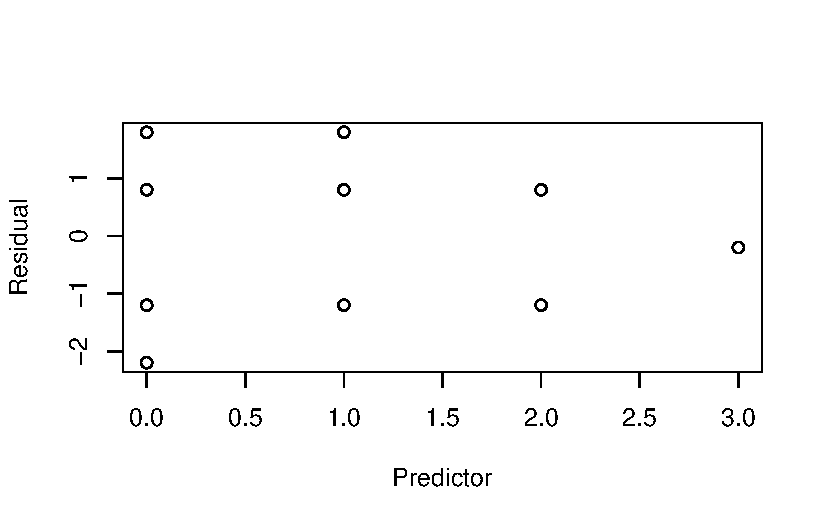
\includegraphics{sta9700_ch3_hw_files/figure-pdf/unnamed-chunk-7-1.pdf}

}

\end{figure}

Plot of residuals against fitted values

\begin{Shaded}
\begin{Highlighting}[]
\FunctionTok{plot}\NormalTok{(}\FunctionTok{residuals}\NormalTok{(airfreight.lm) }\SpecialCharTok{\textasciitilde{}} \FunctionTok{fitted.values}\NormalTok{(airfreight.lm),}
     \AttributeTok{xlab =} \StringTok{"Fitted value"}\NormalTok{, }\AttributeTok{ylab =} \StringTok{"Residual"}\NormalTok{)}
\end{Highlighting}
\end{Shaded}

\begin{figure}[H]

{\centering 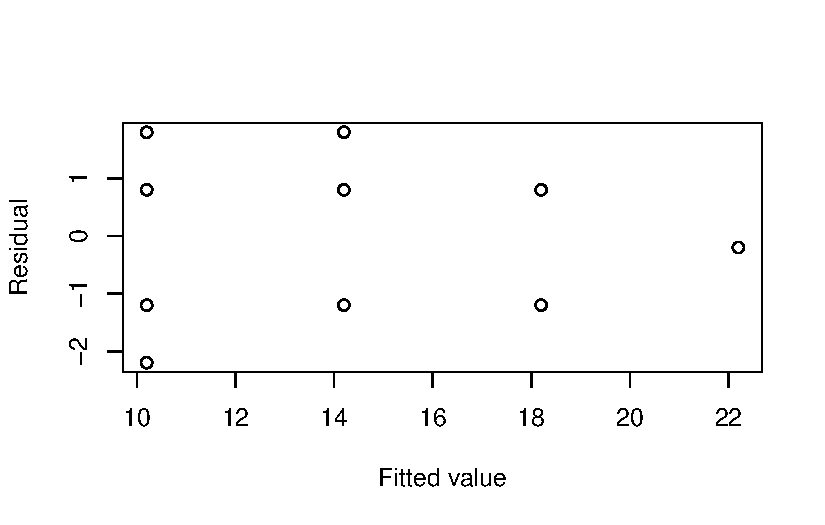
\includegraphics{sta9700_ch3_hw_files/figure-pdf/unnamed-chunk-8-1.pdf}

}

\end{figure}

\textbf{f.~Prepare a time plot of the residuals. What information is
provided by your plot?}

Sequence plot of residuals

\begin{Shaded}
\begin{Highlighting}[]
\FunctionTok{plot}\NormalTok{(airfreight.lm}\SpecialCharTok{$}\NormalTok{residuals,}
     \AttributeTok{type =} \StringTok{"l"}\NormalTok{,}
     \AttributeTok{xlab =} \StringTok{"Production run"}\NormalTok{,}
     \AttributeTok{ylab =} \StringTok{"Residual"}\NormalTok{)}
\FunctionTok{abline}\NormalTok{(}\AttributeTok{h =} \DecValTok{0}\NormalTok{)}
\end{Highlighting}
\end{Shaded}

\begin{figure}[H]

{\centering 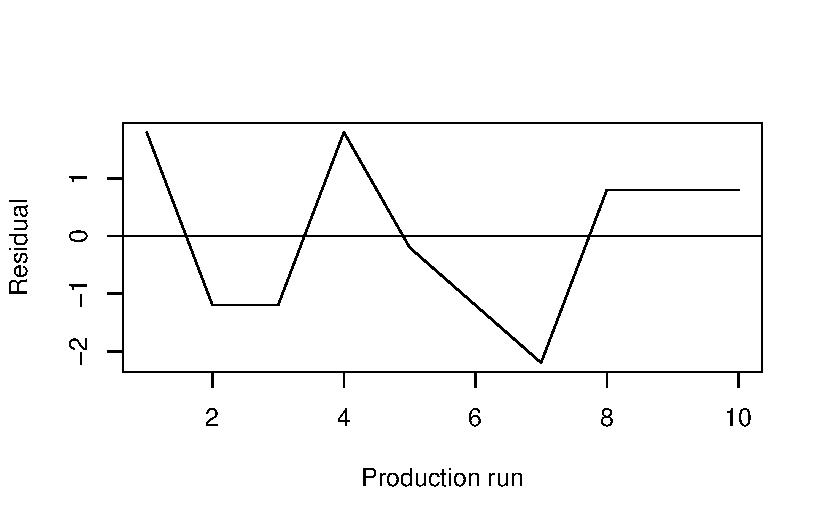
\includegraphics{sta9700_ch3_hw_files/figure-pdf/unnamed-chunk-9-1.pdf}

}

\end{figure}

\begin{Shaded}
\begin{Highlighting}[]
\FunctionTok{par}\NormalTok{(}\AttributeTok{mfrow =} \FunctionTok{c}\NormalTok{(}\DecValTok{2}\NormalTok{, }\DecValTok{2}\NormalTok{))}
\FunctionTok{plot}\NormalTok{(airfreight.lm)}
\end{Highlighting}
\end{Shaded}

\begin{figure}[H]

{\centering 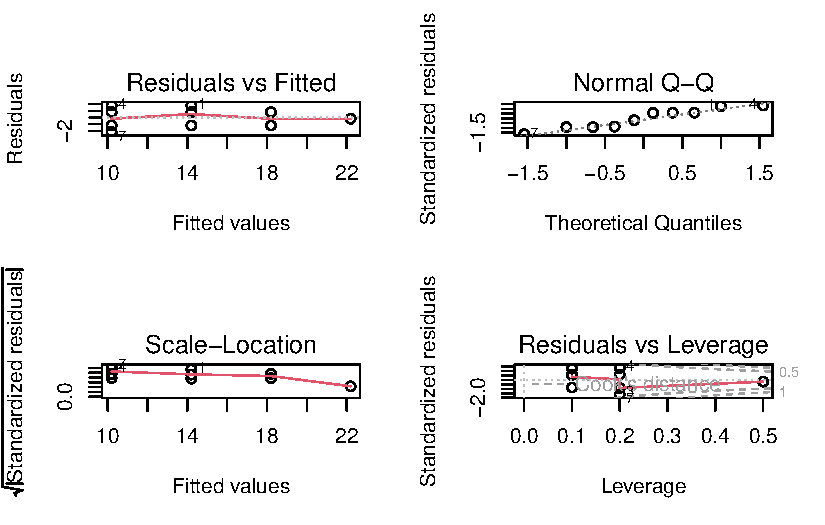
\includegraphics{sta9700_ch3_hw_files/figure-pdf/unnamed-chunk-10-1.pdf}

}

\end{figure}

Plot of semistudentized residuals against fitted values

\begin{Shaded}
\begin{Highlighting}[]
\FunctionTok{plot}\NormalTok{(airfreight.lm}\SpecialCharTok{$}\NormalTok{residuals}\SpecialCharTok{/}\FunctionTok{summary}\NormalTok{(airfreight.lm)}\SpecialCharTok{$}\NormalTok{sigma }\SpecialCharTok{\textasciitilde{}}\NormalTok{ airfreight.lm}\SpecialCharTok{$}\NormalTok{fitted.values, }
     \AttributeTok{xlab =} \StringTok{"Fitted value"}\NormalTok{, }\AttributeTok{ylab =} \StringTok{"Semistudentized residual"}\NormalTok{)}
\end{Highlighting}
\end{Shaded}

\begin{figure}[H]

{\centering 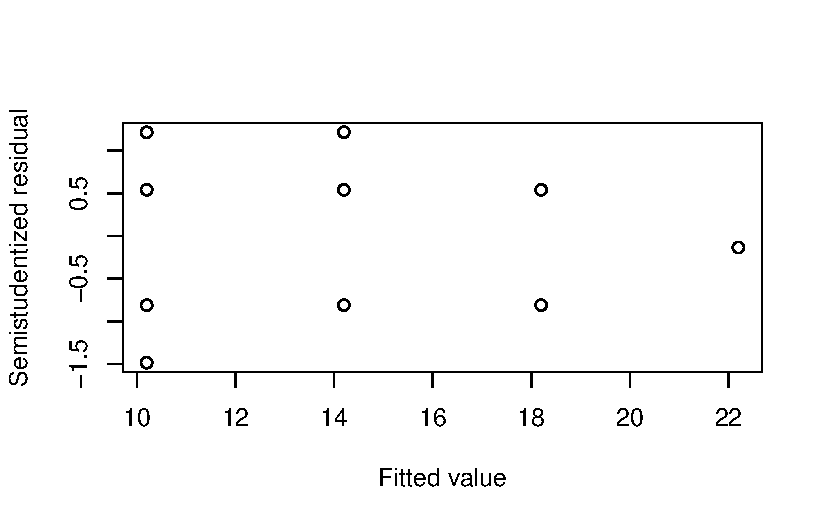
\includegraphics{sta9700_ch3_hw_files/figure-pdf/unnamed-chunk-11-1.pdf}

}

\end{figure}

Normal probability plot of residuals

\begin{Shaded}
\begin{Highlighting}[]
\FunctionTok{qqnorm}\NormalTok{(airfreight.lm}\SpecialCharTok{$}\NormalTok{residuals,}
       \AttributeTok{main =} \StringTok{"Normal Q{-}Q plot of residuals"}\NormalTok{) }
\FunctionTok{qqline}\NormalTok{(airfreight.lm}\SpecialCharTok{$}\NormalTok{residuals)}
\end{Highlighting}
\end{Shaded}

\begin{figure}[H]

{\centering 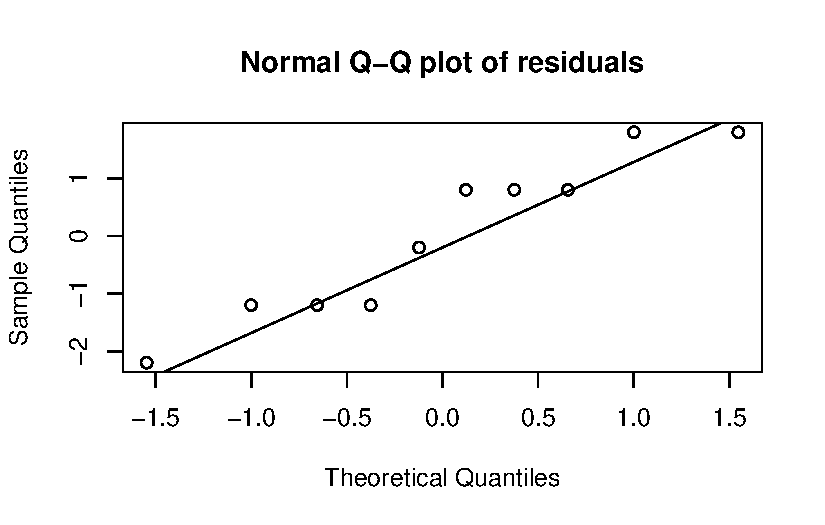
\includegraphics{sta9700_ch3_hw_files/figure-pdf/unnamed-chunk-12-1.pdf}

}

\end{figure}

\textbf{d.} Plot the residuals \(\e_{i}\) against \(X_{i}\) to ascertain
whether any departures from regression model (21.) are evident. What is
your conclusion?

\begin{Shaded}
\begin{Highlighting}[]
\FunctionTok{par}\NormalTok{(}\AttributeTok{mfrow =} \FunctionTok{c}\NormalTok{(}\DecValTok{2}\NormalTok{,}\DecValTok{2}\NormalTok{))}
\FunctionTok{plot}\NormalTok{(airfreight.lm)}
\end{Highlighting}
\end{Shaded}

\begin{figure}[H]

{\centering 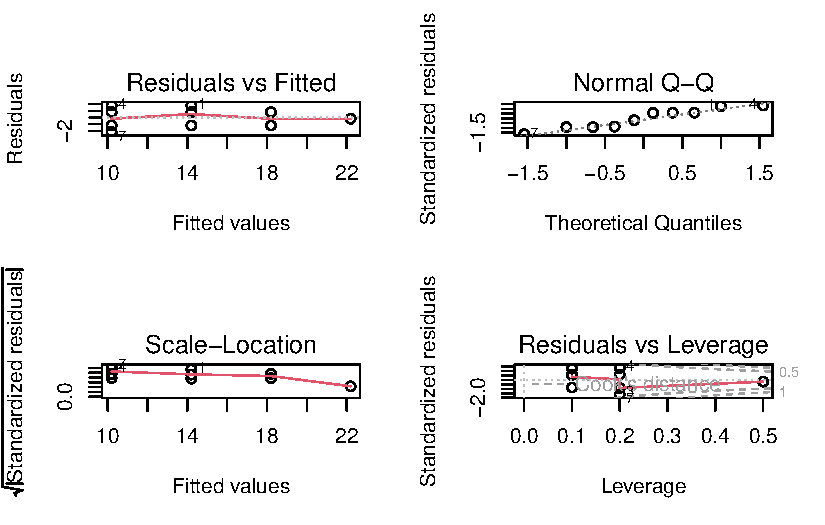
\includegraphics{sta9700_ch3_hw_files/figure-pdf/unnamed-chunk-13-1.pdf}

}

\end{figure}

\textbf{f.} Prepare a time plot of the residuals. what information is
provided by your plot?

\textbf{3.13} Refer to \textbf{Copier maintenance} Problem 1.20.

\begin{Shaded}
\begin{Highlighting}[]
\NormalTok{copier }\OtherTok{\textless{}{-}} \FunctionTok{read.csv}\NormalTok{(}\StringTok{"Copier.csv"}\NormalTok{)}
\end{Highlighting}
\end{Shaded}

\begin{Shaded}
\begin{Highlighting}[]
\NormalTok{copier}
\end{Highlighting}
\end{Shaded}

\begin{verbatim}
     Y  X
1   20  2
2   60  4
3   46  3
4   41  2
5   12  1
6  137 10
7   68  5
8   89  5
9    4  1
10  32  2
11 144  9
12 156 10
13  93  6
14  36  3
15  72  4
16 100  8
17 105  7
18 131  8
19 127 10
20  57  4
21  66  5
22 101  7
23 109  7
24  74  5
25 134  9
26 112  7
27  18  2
28  73  5
29 111  7
30  96  6
31 123  8
32  90  5
33  20  2
34  28  2
35   3  1
36  57  4
37  86  5
38 132  9
39 112  7
40  27  1
41 131  9
42  34  2
43  27  2
44  61  4
45  77  5
\end{verbatim}

\textbf{a.} What are the alternative conclusions when testing for lack
of fit of a linear regression function?

The alternative conclusions when testing for a lack of fit of a linear
regression function are the following:

\begin{enumerate}
\def\labelenumi{\arabic{enumi}.}
\tightlist
\item
  The regression of the function is not linear.
\item
  The error terms do not have a constant variance.
\item
  The error terms are not independent.
\item
  The model fits all but one or a few outlier observations.
\item
  The error terms are not normally distrusted.
\item
  One or several important predictor variables have been omitted from
  the model.
\end{enumerate}

\emph{Nonlinearity of Regression Function} \emph{Nonconstancy of error
variance} \emph{Presence of Outliers} \emph{Nonindependence of error
terms}

\(H_{0}: E{Y} = \beta_{0} + \beta_{1} X\)
\(H_{a}: E{Y} \neq \beta_{0} + \beta_{1} X\)

\textbf{b.} Perform the test indicated in part (a). Control the risk of
Type I error at 0.05. State the decision rule and conclusion.

\begin{Shaded}
\begin{Highlighting}[]
\NormalTok{copier.lm }\OtherTok{\textless{}{-}} \FunctionTok{lm}\NormalTok{(Y }\SpecialCharTok{\textasciitilde{}}\NormalTok{ X, }\AttributeTok{data =}\NormalTok{ copier)}
\FunctionTok{plot}\NormalTok{(Y }\SpecialCharTok{\textasciitilde{}}\NormalTok{ X, }\AttributeTok{data =}\NormalTok{ copier)}
\FunctionTok{abline}\NormalTok{(copier.lm, }\AttributeTok{col=}\StringTok{"red"}\NormalTok{)}
\end{Highlighting}
\end{Shaded}

\begin{figure}[H]

{\centering 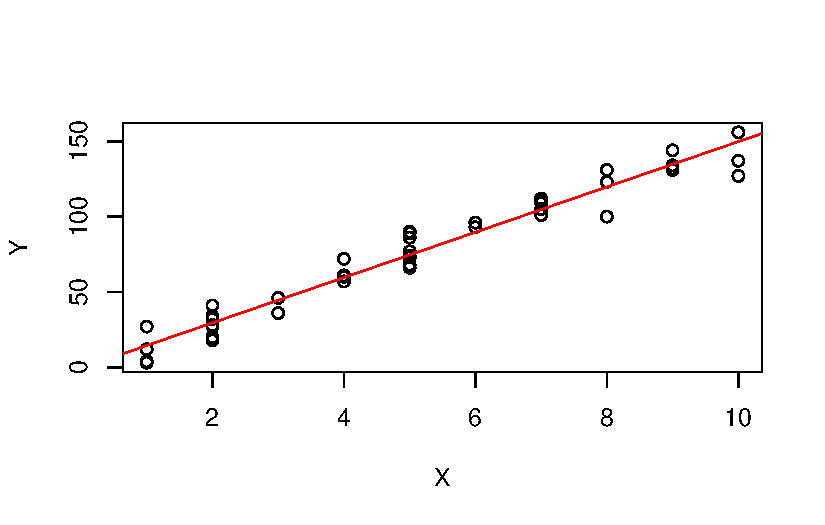
\includegraphics{sta9700_ch3_hw_files/figure-pdf/unnamed-chunk-16-1.pdf}

}

\end{figure}

\emph{F}-test for lack of fit

\begin{Shaded}
\begin{Highlighting}[]
\FunctionTok{anova}\NormalTok{(copier.lm, }\FunctionTok{lm}\NormalTok{(Y }\SpecialCharTok{\textasciitilde{}} \FunctionTok{factor}\NormalTok{(X), }\AttributeTok{data =}\NormalTok{ copier))}
\end{Highlighting}
\end{Shaded}

\begin{verbatim}
Analysis of Variance Table

Model 1: Y ~ X
Model 2: Y ~ factor(X)
  Res.Df    RSS Df Sum of Sq      F Pr(>F)
1     43 3416.4                           
2     35 2797.7  8    618.72 0.9676 0.4766
\end{verbatim}

\begin{Shaded}
\begin{Highlighting}[]
\FunctionTok{anova}\NormalTok{(copier.lm, }\AttributeTok{data =}\NormalTok{ copier)}
\end{Highlighting}
\end{Shaded}

\begin{verbatim}
Warning in anova.lmlist(object, ...): models with response '"NULL"' removed
because response differs from model 1
\end{verbatim}

\begin{verbatim}
Analysis of Variance Table

Response: Y
          Df Sum Sq Mean Sq F value    Pr(>F)    
X          1  76960   76960  968.66 < 2.2e-16 ***
Residuals 43   3416      79                      
---
Signif. codes:  0 '***' 0.001 '**' 0.01 '*' 0.05 '.' 0.1 ' ' 1
\end{verbatim}

\textbf{RSS} = \emph{SSPE} = 2797.7 \textbf{Sum of Sq} = \textbf{SSLF} =
618.72

\(F^{*} = (SSLF/c - 2) / (SSPE / n - c) = MSLF / MSPE\)

\(F^{*} = (618.719/8) / (2797.66 / 35) = 0.967557\)

\(F(0.95; 8; 35) = 2.21668\)

If \(F^{*} \leq 2.21668\), conclude \(H_{0}\), otherwise \(H_{a}\).
Conclude \(H_{0}\)

\(SSPE = \sum\sum (Y_{ij} - \hat Y_{j})^2\) \(df = n - c\)
\(MSLF = SSLF/c - 2\) Number of groups minus 2

\(SSLF = \sum\sum (\hat Y_{j} - \hat Y_{ij})^2\) \(df = c - 2\)
\(MSPE = SSPE/n - c\) Total observations minus number of groups

\textbf{c.} \textbf{Sales growth.} A marketing researcher studied annual
sales of a product that had been introduced 10 years ago. The data are
as follows, where \(X\) is the year (coded) and \(Y\) is sales in
thousands of units:

\begin{longtable}[]{@{}lllllllllll@{}}
\caption{Question 3.17 Sales growth}\tabularnewline
\toprule()
i: & 1 & 2 & 3 & 4 & 5 & 6 & 7 & 8 & 9 & 10 \\
\midrule()
\endfirsthead
\toprule()
i: & 1 & 2 & 3 & 4 & 5 & 6 & 7 & 8 & 9 & 10 \\
\midrule()
\endhead
\(X_{i}\): & 0 & 1 & 2 & 3 & 4 & 5 & 6 & 7 & 8 & 9 \\
\(Y_{i}\): & 98 & 135 & 162 & 178 & 221 & 232 & 283 & 300 & 374 & 395 \\
\bottomrule()
\end{longtable}

\begin{Shaded}
\begin{Highlighting}[]
\NormalTok{sales }\OtherTok{\textless{}{-}}
  \FunctionTok{data.frame}\NormalTok{(}
  \AttributeTok{x =} \FunctionTok{c}\NormalTok{(}\DecValTok{0}\NormalTok{, }\DecValTok{1}\NormalTok{, }\DecValTok{2}\NormalTok{, }\DecValTok{3}\NormalTok{, }\DecValTok{4}\NormalTok{, }\DecValTok{5}\NormalTok{, }\DecValTok{6}\NormalTok{, }\DecValTok{7}\NormalTok{, }\DecValTok{8}\NormalTok{, }\DecValTok{9}\NormalTok{),}
  \AttributeTok{y =} \FunctionTok{c}\NormalTok{(}\DecValTok{98}\NormalTok{, }\DecValTok{135}\NormalTok{, }\DecValTok{162}\NormalTok{, }\DecValTok{178}\NormalTok{, }\DecValTok{221}\NormalTok{, }\DecValTok{232}\NormalTok{, }\DecValTok{283}\NormalTok{, }\DecValTok{300}\NormalTok{, }\DecValTok{374}\NormalTok{, }\DecValTok{395}\NormalTok{)}
\NormalTok{  )}
\end{Highlighting}
\end{Shaded}

\begin{Shaded}
\begin{Highlighting}[]
\NormalTok{sales}
\end{Highlighting}
\end{Shaded}

\begin{verbatim}
   x   y
1  0  98
2  1 135
3  2 162
4  3 178
5  4 221
6  5 232
7  6 283
8  7 300
9  8 374
10 9 395
\end{verbatim}

\textbf{a.} Prepare a scatter plot of the data. Does a linear relation
appear to be accurate?

\begin{Shaded}
\begin{Highlighting}[]
\NormalTok{sales.lm }\OtherTok{\textless{}{-}} \FunctionTok{lm}\NormalTok{(y }\SpecialCharTok{\textasciitilde{}}\NormalTok{ x, }\AttributeTok{data =}\NormalTok{ sales)}
\end{Highlighting}
\end{Shaded}

\begin{Shaded}
\begin{Highlighting}[]
\FunctionTok{plot}\NormalTok{(y }\SpecialCharTok{\textasciitilde{}}\NormalTok{ x, }\AttributeTok{data =}\NormalTok{ sales)}
\FunctionTok{abline}\NormalTok{(sales.lm, }\AttributeTok{col=}\StringTok{"red"}\NormalTok{)}
\end{Highlighting}
\end{Shaded}

\begin{figure}[H]

{\centering 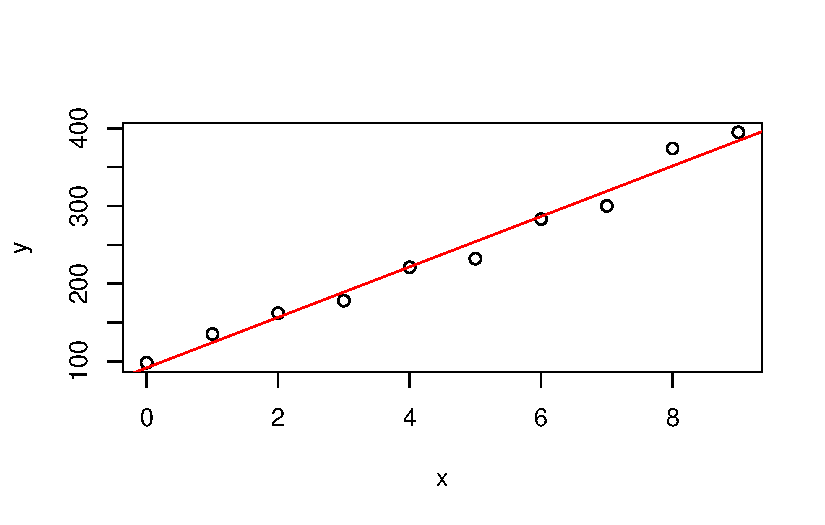
\includegraphics{sta9700_ch3_hw_files/figure-pdf/unnamed-chunk-22-1.pdf}

}

\end{figure}

\textbf{b.} Use the Box-Cox procedure and standardization (3.36) to find
an appropriate power transformation of \(Y\). Evaluate \(SSE\) for
\(\lambda = 0.3, 0.4, 0.5, 0.6, 0.7\).

What transformation of Y is suggested?

Transformations on Y

\hypertarget{box-cox-transformation}{%
\section{Box-Cox transformation}\label{box-cox-transformation}}

\begin{Shaded}
\begin{Highlighting}[]
\FunctionTok{boxcox.sse}\NormalTok{(sales[,}\DecValTok{1}\NormalTok{],sales[,}\DecValTok{2}\NormalTok{],}\AttributeTok{l=}\FunctionTok{seq}\NormalTok{(}\SpecialCharTok{{-}}\DecValTok{2}\NormalTok{,}\DecValTok{1}\NormalTok{,}\FloatTok{0.1}\NormalTok{))}
\end{Highlighting}
\end{Shaded}

\begin{figure}[H]

{\centering 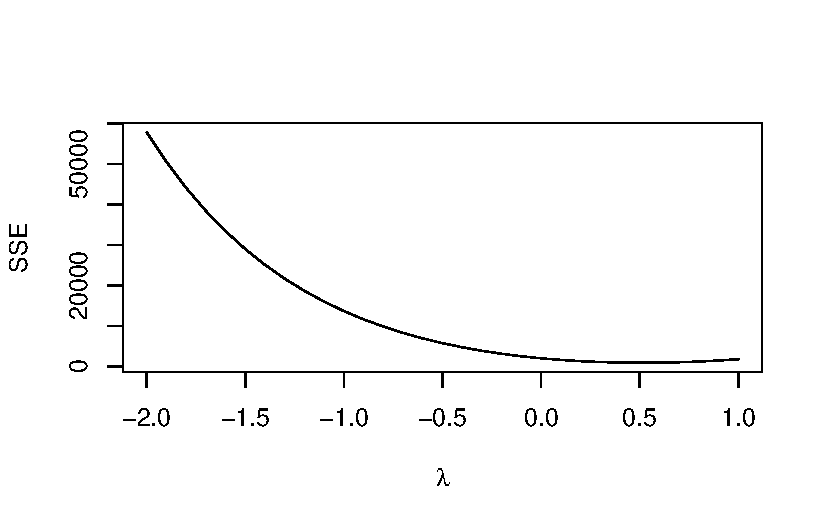
\includegraphics{sta9700_ch3_hw_files/figure-pdf/unnamed-chunk-23-1.pdf}

}

\end{figure}

\begin{verbatim}
   lambda        SSE
1    -2.0 57788.3511
2    -1.9 50489.6939
3    -1.8 44054.1816
4    -1.7 38379.8733
5    -1.6 33377.2323
6    -1.5 28967.6103
7    -1.4 25081.9206
8    -1.3 21659.4777
9    -1.2 18646.9811
10   -1.1 15997.6263
11   -1.0 13670.3269
12   -0.9 11629.0334
13   -0.8  9842.1378
14   -0.7  8281.9520
15   -0.6  6924.2528
16   -0.5  5747.8831
17   -0.4  4734.4047
18   -0.3  3867.7951
19   -0.2  3134.1829
20   -0.1  2521.6190
31    0.0  2019.8767
21    0.1  1620.2804
22    0.2  1315.5569
23    0.3  1099.7093
24    0.4   967.9088
25    0.5   916.4048
26    0.6   942.4498
27    0.7  1044.2384
28    0.8  1220.8598
29    0.9  1472.2614
30    1.0  1799.2242
\end{verbatim}

\begin{longtable}[]{@{}llllll@{}}
\toprule()
\lambda: & 0.3 & 0.4 & 0.5 & 0.6 & 0.7 \\
\midrule()
\endhead
\(SSE\): & 1099.7 & 967.9 & 916.4 & 942.4 & 1044.2 \\
\bottomrule()
\end{longtable}

\textbf{c.} Use the transformation \(Y' = \sqrt Y\) and obtain the
estimated linear regression function for the transformed data.

\begin{Shaded}
\begin{Highlighting}[]
\FunctionTok{plot}\NormalTok{(y }\SpecialCharTok{\textasciitilde{}}\NormalTok{ x, }\AttributeTok{data =}\NormalTok{ sales)}
\end{Highlighting}
\end{Shaded}

\begin{figure}[H]

{\centering 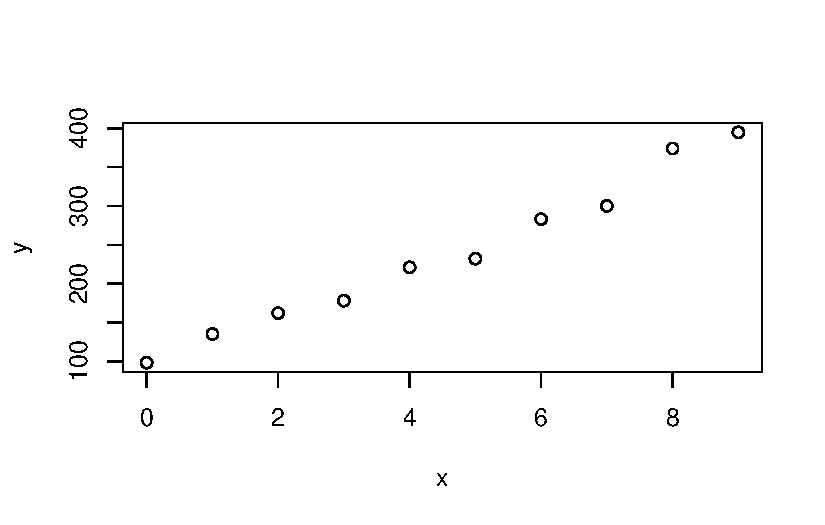
\includegraphics{sta9700_ch3_hw_files/figure-pdf/unnamed-chunk-24-1.pdf}

}

\end{figure}

\begin{Shaded}
\begin{Highlighting}[]
\NormalTok{sales.lm\_sqrt }\OtherTok{\textless{}{-}} \FunctionTok{lm}\NormalTok{(}\FunctionTok{sqrt}\NormalTok{(y) }\SpecialCharTok{\textasciitilde{}}\NormalTok{ x, }\AttributeTok{data =}\NormalTok{ sales)}
\end{Highlighting}
\end{Shaded}

\begin{Shaded}
\begin{Highlighting}[]
\FunctionTok{plot}\NormalTok{(}\FunctionTok{sqrt}\NormalTok{(y) }\SpecialCharTok{\textasciitilde{}}\NormalTok{ x, }\AttributeTok{data =}\NormalTok{ sales)}
\end{Highlighting}
\end{Shaded}

\begin{figure}[H]

{\centering 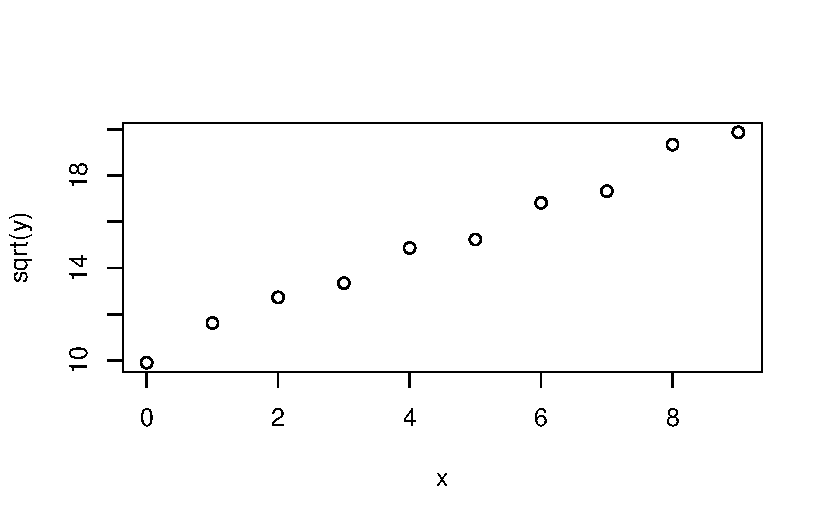
\includegraphics{sta9700_ch3_hw_files/figure-pdf/unnamed-chunk-26-1.pdf}

}

\end{figure}

\begin{Shaded}
\begin{Highlighting}[]
\FunctionTok{par}\NormalTok{(}\AttributeTok{mfrow =} \FunctionTok{c}\NormalTok{(}\DecValTok{2}\NormalTok{, }\DecValTok{2}\NormalTok{))}
\FunctionTok{plot}\NormalTok{(sales.lm\_sqrt)}
\end{Highlighting}
\end{Shaded}

\begin{figure}[H]

{\centering 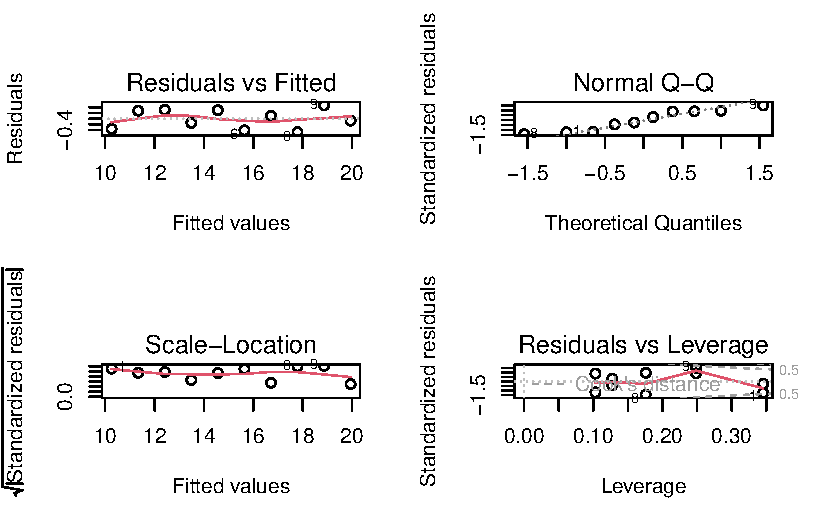
\includegraphics{sta9700_ch3_hw_files/figure-pdf/unnamed-chunk-27-1.pdf}

}

\end{figure}

\begin{Shaded}
\begin{Highlighting}[]
\FunctionTok{summary}\NormalTok{(sales.lm\_sqrt)}
\end{Highlighting}
\end{Shaded}

\begin{verbatim}

Call:
lm(formula = sqrt(y) ~ x, data = sales)

Residuals:
     Min       1Q   Median       3Q      Max 
-0.47447 -0.30811  0.01549  0.29541  0.46781 

Coefficients:
            Estimate Std. Error t value Pr(>|t|)    
(Intercept) 10.26093    0.21290   48.20 3.80e-11 ***
x            1.07629    0.03988   26.99 3.83e-09 ***
---
Signif. codes:  0 '***' 0.001 '**' 0.01 '*' 0.05 '.' 0.1 ' ' 1

Residual standard error: 0.3622 on 8 degrees of freedom
Multiple R-squared:  0.9891,    Adjusted R-squared:  0.9878 
F-statistic: 728.4 on 1 and 8 DF,  p-value: 3.826e-09
\end{verbatim}

\(Y = 1.07629X + 10.26093\)

\begin{Shaded}
\begin{Highlighting}[]
\FunctionTok{plot}\NormalTok{(sales.lm}\SpecialCharTok{$}\NormalTok{residuals }\SpecialCharTok{\textasciitilde{}}\NormalTok{ sales}\SpecialCharTok{$}\NormalTok{x, }\AttributeTok{xlab =} \StringTok{"x"}\NormalTok{, }\AttributeTok{ylab =} \StringTok{"Residual"}\NormalTok{)}
\FunctionTok{abline}\NormalTok{(}\AttributeTok{h =} \DecValTok{0}\NormalTok{)}
\end{Highlighting}
\end{Shaded}

\begin{figure}[H]

{\centering 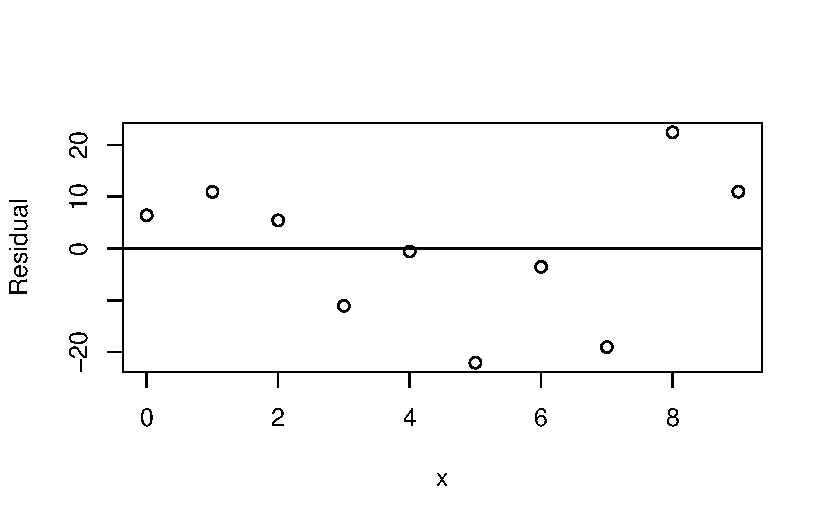
\includegraphics{sta9700_ch3_hw_files/figure-pdf/unnamed-chunk-29-1.pdf}

}

\end{figure}

\begin{Shaded}
\begin{Highlighting}[]
\FunctionTok{plot}\NormalTok{(sales.lm}\SpecialCharTok{$}\NormalTok{residuals }\SpecialCharTok{\textasciitilde{}}\NormalTok{ sales}\SpecialCharTok{$}\NormalTok{x, }\AttributeTok{xlab =} \StringTok{"x"}\NormalTok{, }\AttributeTok{ylab =} \StringTok{"Residual"}\NormalTok{)}
\end{Highlighting}
\end{Shaded}

\begin{figure}[H]

{\centering 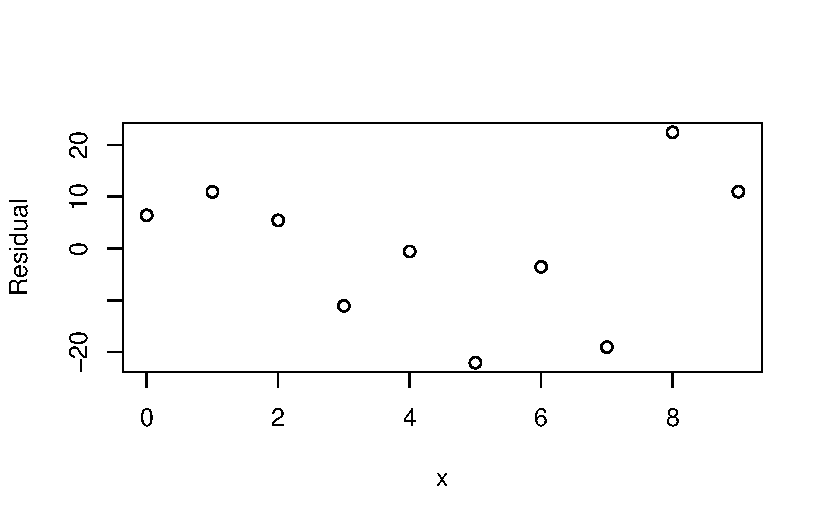
\includegraphics{sta9700_ch3_hw_files/figure-pdf/unnamed-chunk-30-1.pdf}

}

\end{figure}

\begin{Shaded}
\begin{Highlighting}[]
\FunctionTok{plot}\NormalTok{(sales.lm}\SpecialCharTok{$}\NormalTok{residuals }\SpecialCharTok{\textasciitilde{}}\NormalTok{ sales.lm}\SpecialCharTok{$}\NormalTok{fitted.values, }
     \AttributeTok{xlab =} \StringTok{"Fitted value"}\NormalTok{, }\AttributeTok{ylab =} \StringTok{"Residual"}\NormalTok{)}
\end{Highlighting}
\end{Shaded}

\begin{figure}[H]

{\centering 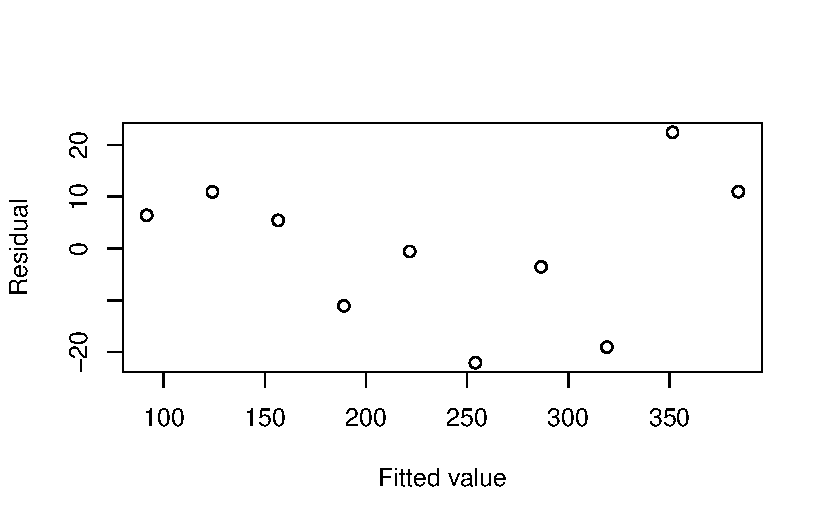
\includegraphics{sta9700_ch3_hw_files/figure-pdf/unnamed-chunk-31-1.pdf}

}

\end{figure}

\textbf{d.} Plot the estimated regression line and transformed data.
Does the regression line appear to be a good fit to the transformed
data?

\begin{Shaded}
\begin{Highlighting}[]
\FunctionTok{plot}\NormalTok{(}\FunctionTok{sqrt}\NormalTok{(y) }\SpecialCharTok{\textasciitilde{}}\NormalTok{ x, }\AttributeTok{data =}\NormalTok{ sales)}
\end{Highlighting}
\end{Shaded}

\begin{figure}[H]

{\centering 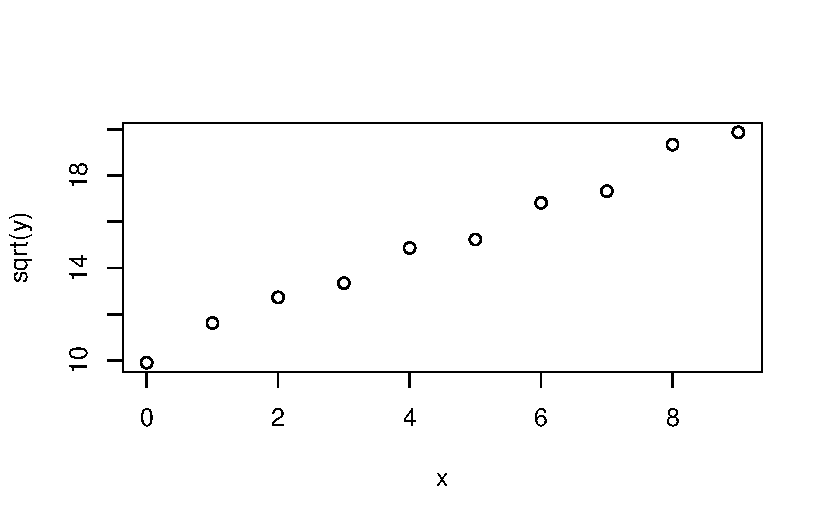
\includegraphics{sta9700_ch3_hw_files/figure-pdf/unnamed-chunk-32-1.pdf}

}

\end{figure}

\textbf{e.} Obtain the residuals and plot them against the fitted
values. Also prepare a normal probability plot. What do your plots show?

Residuals

\begin{Shaded}
\begin{Highlighting}[]
\NormalTok{sales.lm\_sqrt}\SpecialCharTok{$}\NormalTok{residuals }
\end{Highlighting}
\end{Shaded}

\begin{verbatim}
          1           2           3           4           5           6 
-0.36143656  0.28172678  0.31440703 -0.14814273  0.29997018 -0.41084412 
          7           8           9          10 
 0.10392174 -0.47446579  0.46781397 -0.07295049 
\end{verbatim}

Plot of residuals against fitted values

\begin{Shaded}
\begin{Highlighting}[]
\FunctionTok{plot}\NormalTok{(}\FunctionTok{residuals}\NormalTok{(sales.lm\_sqrt) }\SpecialCharTok{\textasciitilde{}} \FunctionTok{fitted.values}\NormalTok{(sales.lm\_sqrt),}
     \AttributeTok{xlab =} \StringTok{"Fitted value"}\NormalTok{, }\AttributeTok{ylab =} \StringTok{"Residual"}\NormalTok{)}
\end{Highlighting}
\end{Shaded}

\begin{figure}[H]

{\centering 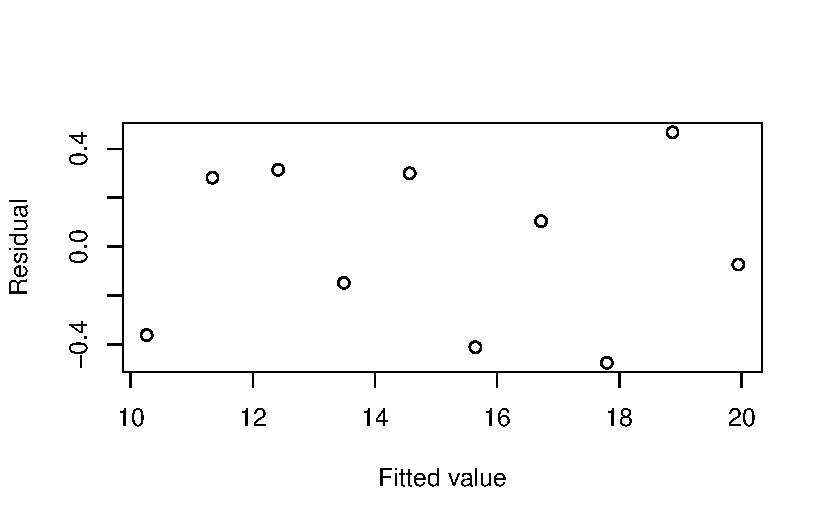
\includegraphics{sta9700_ch3_hw_files/figure-pdf/unnamed-chunk-34-1.pdf}

}

\end{figure}

\begin{Shaded}
\begin{Highlighting}[]
\FunctionTok{fitted.values}\NormalTok{(sales.lm\_sqrt)}
\end{Highlighting}
\end{Shaded}

\begin{verbatim}
       1        2        3        4        5        6        7        8 
10.26093 11.33722 12.41352 13.48981 14.56610 15.64239 16.71868 17.79497 
       9       10 
18.87127 19.94756 
\end{verbatim}

\begin{Shaded}
\begin{Highlighting}[]
\NormalTok{expected }\OtherTok{\textless{}{-}} \FunctionTok{data.frame}\NormalTok{(}\AttributeTok{actual =}\NormalTok{ sales}\SpecialCharTok{$}\NormalTok{y, }\AttributeTok{predicted =} \FunctionTok{predict}\NormalTok{(sales.lm\_sqrt))}
\NormalTok{expected}
\end{Highlighting}
\end{Shaded}

\begin{verbatim}
   actual predicted
1      98  10.26093
2     135  11.33722
3     162  12.41352
4     178  13.48981
5     221  14.56610
6     232  15.64239
7     283  16.71868
8     300  17.79497
9     374  18.87127
10    395  19.94756
\end{verbatim}

\begin{Shaded}
\begin{Highlighting}[]
\NormalTok{sales}\SpecialCharTok{$}\NormalTok{Pred }\OtherTok{\textless{}{-}} \FunctionTok{fitted}\NormalTok{(sales.lm\_sqrt)}
\end{Highlighting}
\end{Shaded}

\begin{Shaded}
\begin{Highlighting}[]
\NormalTok{sales}\SpecialCharTok{$}\NormalTok{Pred}
\end{Highlighting}
\end{Shaded}

\begin{verbatim}
 [1] 10.26093 11.33722 12.41352 13.48981 14.56610 15.64239 16.71868 17.79497
 [9] 18.87127 19.94756
\end{verbatim}

\begin{Shaded}
\begin{Highlighting}[]
\NormalTok{sales}\SpecialCharTok{$}\NormalTok{Resid }\OtherTok{\textless{}{-}}\NormalTok{ sales}\SpecialCharTok{$}\NormalTok{y }\SpecialCharTok{{-}}\NormalTok{ sales}\SpecialCharTok{$}\NormalTok{Pred}
\end{Highlighting}
\end{Shaded}

\begin{Shaded}
\begin{Highlighting}[]
\NormalTok{sales}\SpecialCharTok{$}\NormalTok{Resid}
\end{Highlighting}
\end{Shaded}

\begin{verbatim}
 [1]  87.73907 123.66278 149.58648 164.51019 206.43390 216.35761 266.28132
 [8] 282.20503 355.12873 375.05244
\end{verbatim}

\begin{Shaded}
\begin{Highlighting}[]
\NormalTok{sales.sqrt\_qq }\OtherTok{\textless{}{-}} \FunctionTok{qqnorm}\NormalTok{(sales.lm\_sqrt}\SpecialCharTok{$}\NormalTok{residuals, }\AttributeTok{main =} \StringTok{"Normal Q{-}Q plot of residuals"}\NormalTok{)}
\end{Highlighting}
\end{Shaded}

\begin{figure}[H]

{\centering 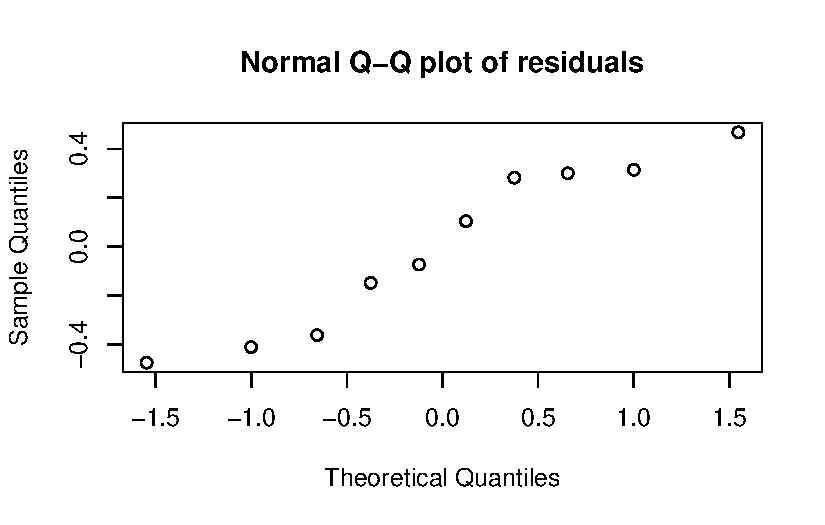
\includegraphics{sta9700_ch3_hw_files/figure-pdf/unnamed-chunk-41-1.pdf}

}

\end{figure}

\begin{longtable}[]{@{}llllll@{}}
\toprule()
\(i\): & 1 & 2 & 3 & 4 & 5 \\
\midrule()
\endhead
\(e_{i}\): & -0.36 & 0.28 & 0.31 & -0.15 & 0.30 \\
\(\hat Y_{i}^{'}\): & 10.26 & 11.34 & 12.41 & 13.49 & 14.57 \\
\emph{Expected value}: & -0.24 & 0.14 & 0.36 & -0.14 & 0.24 \\
\bottomrule()
\end{longtable}

\begin{longtable}[]{@{}llllll@{}}
\toprule()
\(i\): & 6 & 7 & 8 & 9 & 10 \\
\midrule()
\endhead
\(e_{i}\): & -0.41 & 0.10 & 0.47 & 0.47 & -0.07 \\
\(\hat Y_{i}^{'}\): & 15.64 & 16.72 & 17.79 & 18.87 & 19.95 \\
\emph{Expected value}: & -0.36 & 0.04 & -0.56 & 0.56 & -0.04 \\
\bottomrule()
\end{longtable}

\textbf{f.} Express the estimated regression function in original units.

\(Y = (1.07629X + 10.26093)^{2}\)



\end{document}
